\documentclass{beamer}

\mode<presentation>
{
  \usetheme{CambridgeUS}
  \setbeamercovered{invisible}
}

\usepackage[english]{babel}
\usepackage[latin1]{inputenc}
\usepackage{times}
\usepackage[T1]{fontenc} 
% Or whatever. Note that the encoding and the font should match. If T1
% does not look nice, try deleting the line with the fontenc.
\usepackage{amsmath}

\newcommand{\linespace}{\vskip 0.25cm}

% The text in square brackets is the short version of your title and will be used in the
% header/footer depending on your theme.
\title[Graph database analysis of GP dynamics]{Silico-paleontology with graph databases}
%{Using Graph Databases to Explore Genetic Programming Run Dynamics}

% Sub-titles are optional - uncomment and edit the next line if you want one.
\subtitle{Rooting through the relics of digital evolution} 

% The text in square brackets is the short version of your name(s) and will be used in the
% header/footer depending on your theme.
\author[McPhee \& Donatucci]{Nic McPhee \& David Donatucci (w/ Thomas Helmuth)}

% The text in square brackets is the short version of your institution and will be used in the
% header/footer depending on your theme.
\institute[UMN Morris]
{
  Division of Science and Mathematics \\
  University of Minnesota, Morris \\
  Morris, Minnesota, USA \\
}

% The text in square brackets is the short version of the date if you need that.
\date[May 2015, GPTP, Ann Arbor MI] % (optional)
{May 2015 \\ Genetic Programming Theory and Practice \\ University of Michigan \\ Ann Arbor, MI}

% Delete this, if you do not want the table of contents to pop up at
% the beginning of each subsection:
\AtBeginSection[]
{
  \begin{frame}<beamer>
    \frametitle{Outline}
    \tableofcontents[currentsection, hideothersubsections]
  \end{frame}
}

\begin{document}

\begin{frame}
  \titlepage
\end{frame}

% For a 20-25 minute senior seminar talk you probably want something like:
% - Two or three major sections (other than the summary).
% - At *most* three subsections per section.
% - Talk about 30s to 2min per frame. So there should probably be between
%   15 and 30 frames, all told.

\section*{Overview}

\subsection*{The Big Picture}

\begin{frame}
  \frametitle{The Big Picture}
  
  \begin{itemize}
	\item Genetic programming clearly \emph{works}.
	\item But we rarely know \emph{why} or \emph{how}.
	\item Databases allow examination of the internal interactions of a run.
	\item Graph databases better suited for this than relational databases.
	\item Silico-paleontology can help us understand and improve our tools.
  \end{itemize}

\end{frame}

\subsection*{Outline}

\begin{frame}
  \frametitle{Outline}
  \tableofcontents[hideallsubsections]
\end{frame}

\section{What do we know? (And how do we talk about it?)}

\subsection{We throw so much away}

\begin{frame}{We keep/see/share so little}
	
	\begin{columns}
		\begin{column}{0.6 \linewidth}
			EC research has the potential to generate \emph{huge} amounts of data.
			\linespace
			What do we normally do with that data?
			\linespace
			We normally throw it away -- \& paleontologists weep!
			\linespace
			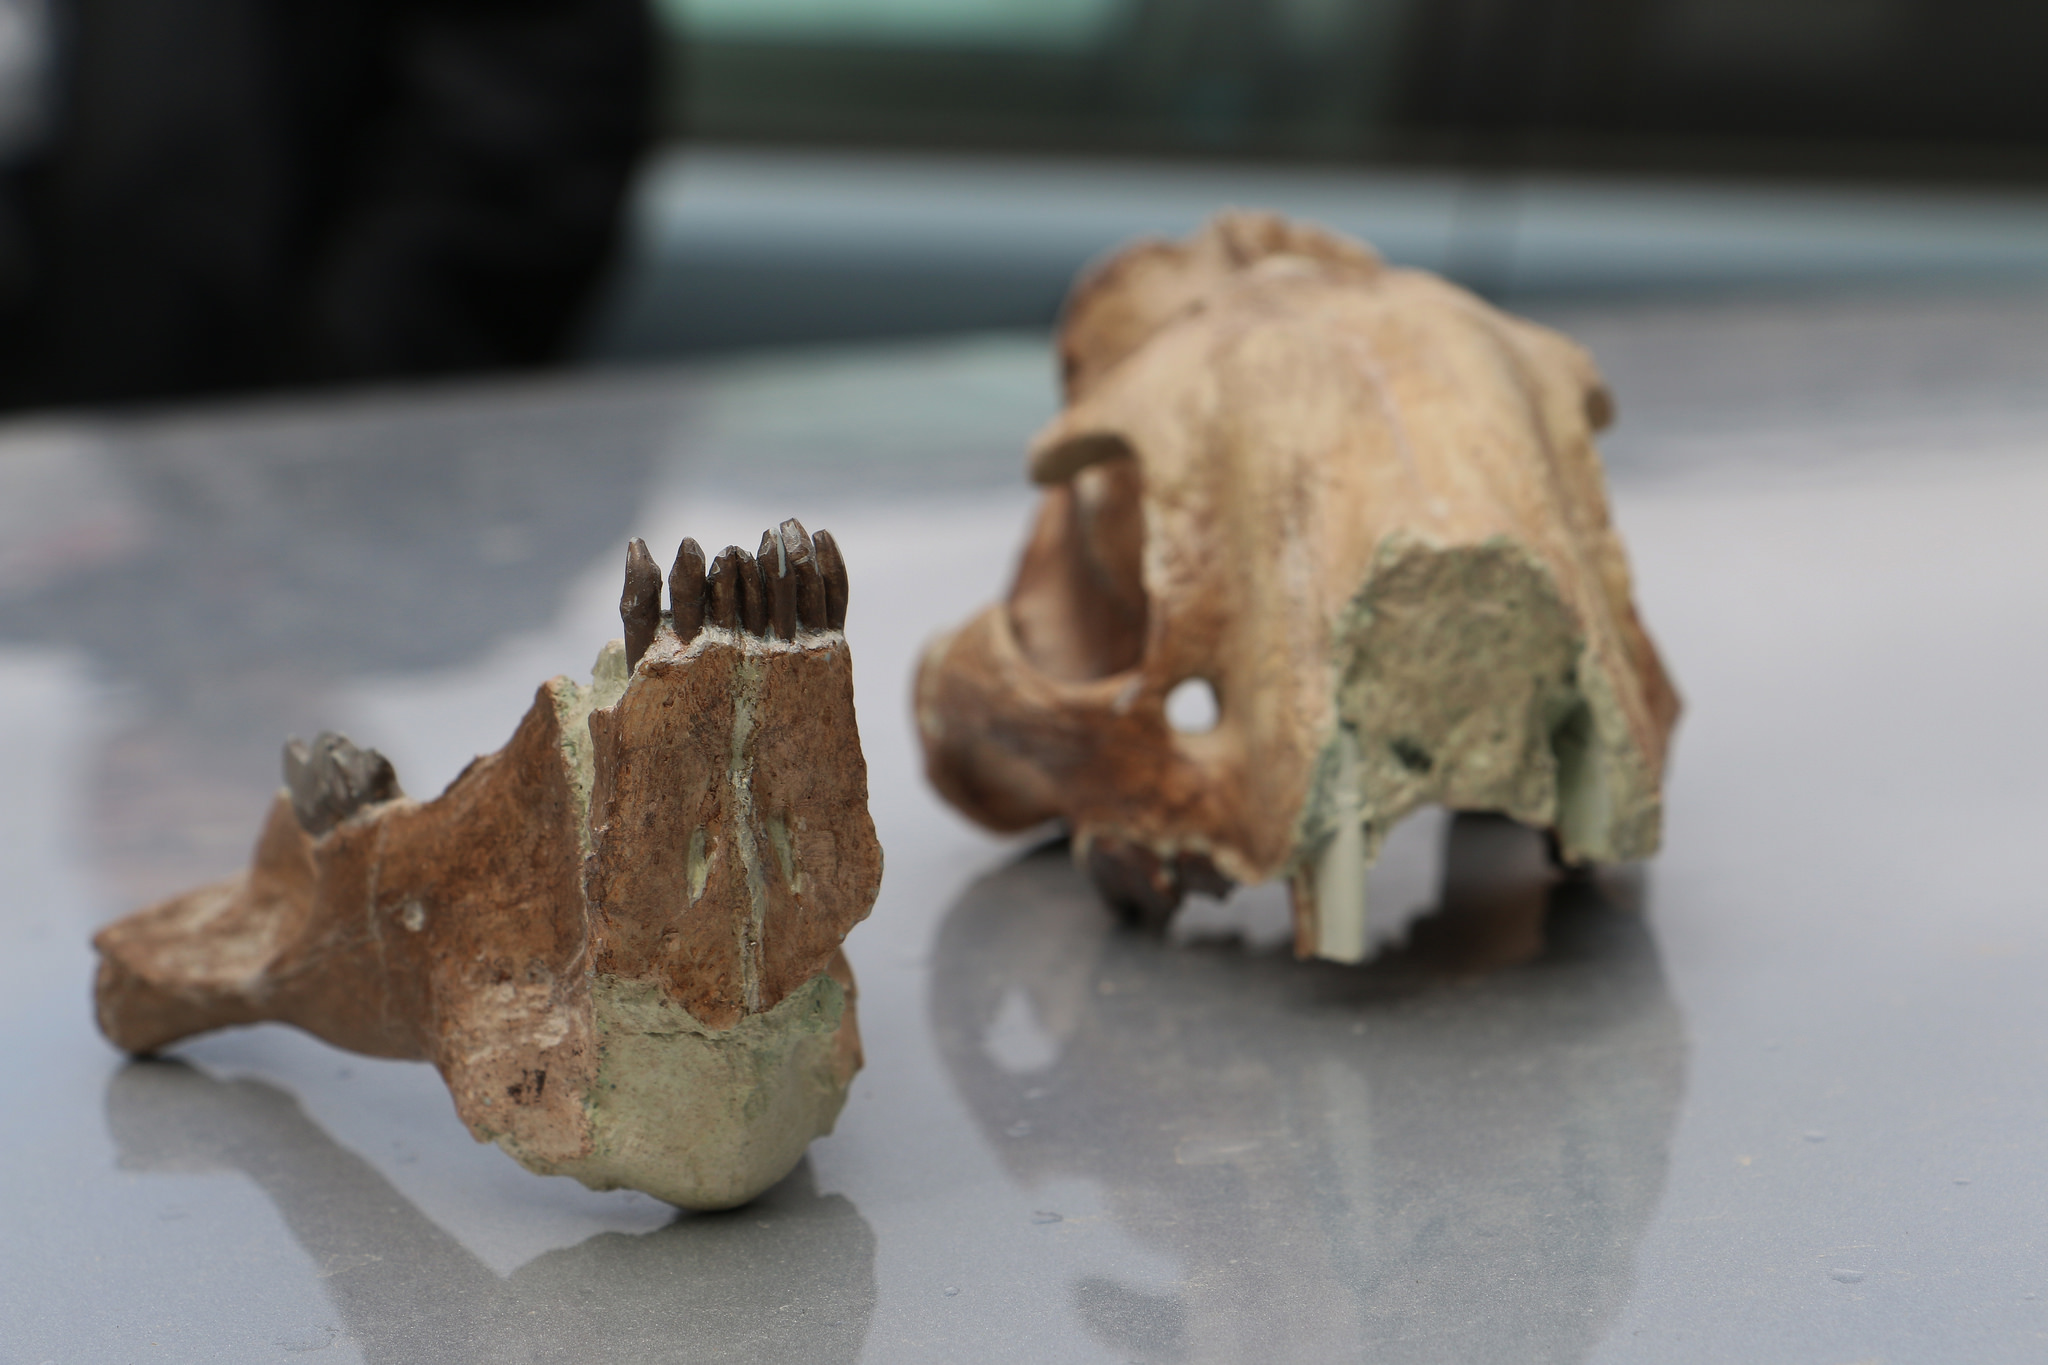
\includegraphics[width = 0.8 \linewidth]{Figures/FossilsMedium.jpg} \\
			\tiny{\url{https://www.flickr.com/photos/blmoregon/14566767645/}}
		\end{column}
		\begin{column}{0.4 \linewidth}
			\includegraphics[height= 0.7 \textheight]{Figures/Abandoned_books.jpg} \\
			\tiny{\url{https://www.flickr.com/photos/nicmcphee/1323950471}}
		\end{column}
	\end{columns}
\end{frame}

\subsection{Summary results are highly lossy}

\begin{frame}{Oooh -- a table of results!}

\begin{columns}
	\begin{column}{0.4 \linewidth}
		\centering
\begin{tabular}{lrrr}
	& \multicolumn{3}{c}{Treatment} \\ \cline{2-4}
	\textbf{Problem} & \textbf{L} & \textbf{T} & \textbf{I} \\
	\hline
	RSWN & 55 & 13 & 17 \\
	SYL & 22 & 1 & 2 \\
	SLB & 75 & 19 & 10 \\
	NTZ & 57 & 15 & 7
\end{tabular}
\end{column}

\begin{column}{0.55 \linewidth}
	\begin{overprint}
		\onslide<1>
		These show successes on 4 problems for 3 different treatments
		\linespace
		L seems to be winning

		\onslide<2>
		But \emph{why?!?!?}		
		\linespace
		What's actually \emph{happening} in all those matings and crossovers and mutations that makes the difference?
	\end{overprint}
\end{column}
\end{columns}
\end{frame}

\subsection{Plots are better (but can still obscure details)}

\begin{frame}{Let's draw pretty pictures}
	
	\begin{columns}
		\begin{column}{0.55 \linewidth}
			\centering
			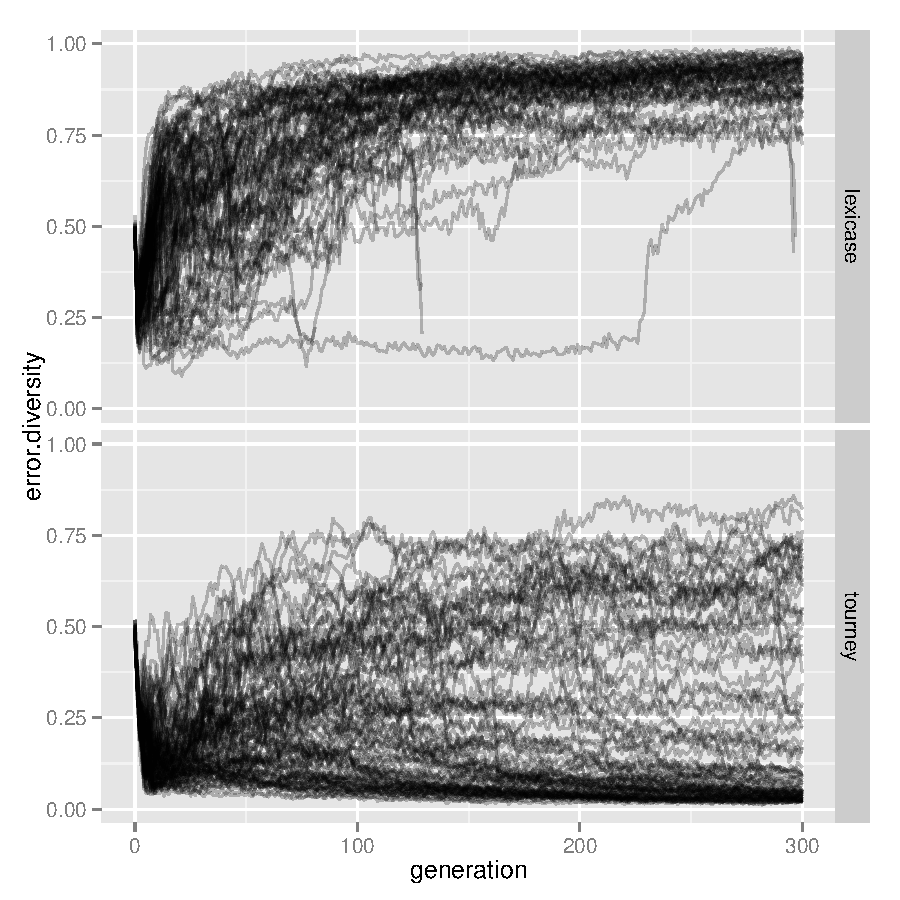
\includegraphics[width = \linewidth]{Figures/rswn_diversity.pdf}
		\end{column}
		
		\begin{column}{0.4 \linewidth}
			\begin{overprint}
				\onslide<1>
				So much more data!
				\linespace
				Diversity over time across all the runs.
				\linespace
				L's diversity (top) is consistently higher than T (bottom).
				\linespace
				That might be important (and supports some hypotheses).
				
				\onslide<2>
				Still, this mushes all the runs together.
				\linespace
				And that likely obscures interesting things.
			\end{overprint}
		\end{column}
	\end{columns}
\end{frame}

\subsection{Can we zoom in to individual runs?}

\begin{frame}{Zooming in}
	
	\begin{columns}
		\begin{column}{0.55 \linewidth}
			\centering
			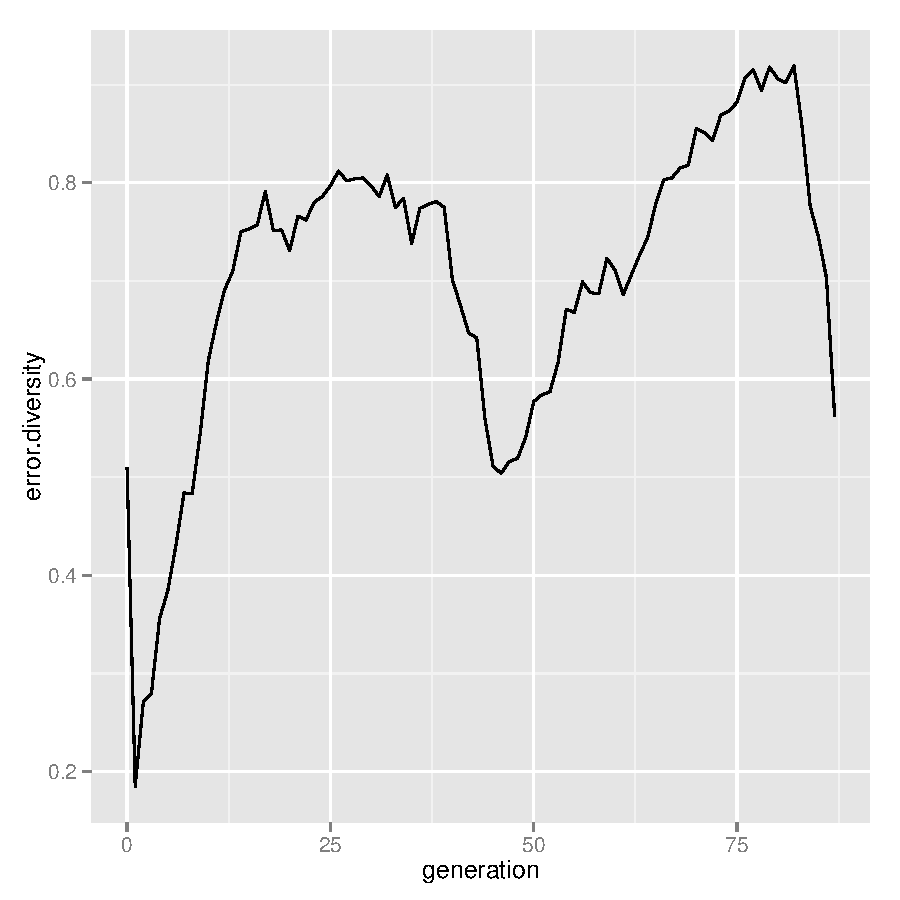
\includegraphics[width = \linewidth]{Figures/run6_lexicase_rswn_diversity.pdf}
		\end{column}
		
		\begin{column}{0.4 \linewidth}
			\begin{overprint}
				\onslide<1>
				Focusing on one successful L run now.
				\linespace
				Three big diversity changes:
				\begin{itemize}
					\item First 15 generations have a sharp drop then steep rise
					\item Around generation 40 a sharp drop and rise
					\item Sharp drop at end just before a solution is found
				\end{itemize}
				
				\onslide<2>
				\emph{What's happening at those sections of the run?}
				\linespace
				We want to be able to dig through a run and see what happened.
			\end{overprint}
		\end{column}
	\end{columns}
\end{frame}

\section[Using a graph DB]{Using a graph database}

\subsection{Goals}

\begin{frame}{Goals}
	\begin{columns}
		\begin{column}{0.6 \linewidth}
					We want to store and analyze \emph{all} the individuals and their relationships.
					\linespace
					Ancestry relationships are naturally modeled with a graph
					\linespace
					So graph databases seem a natural tool for the relationship part.
					\linespace
					\centering
					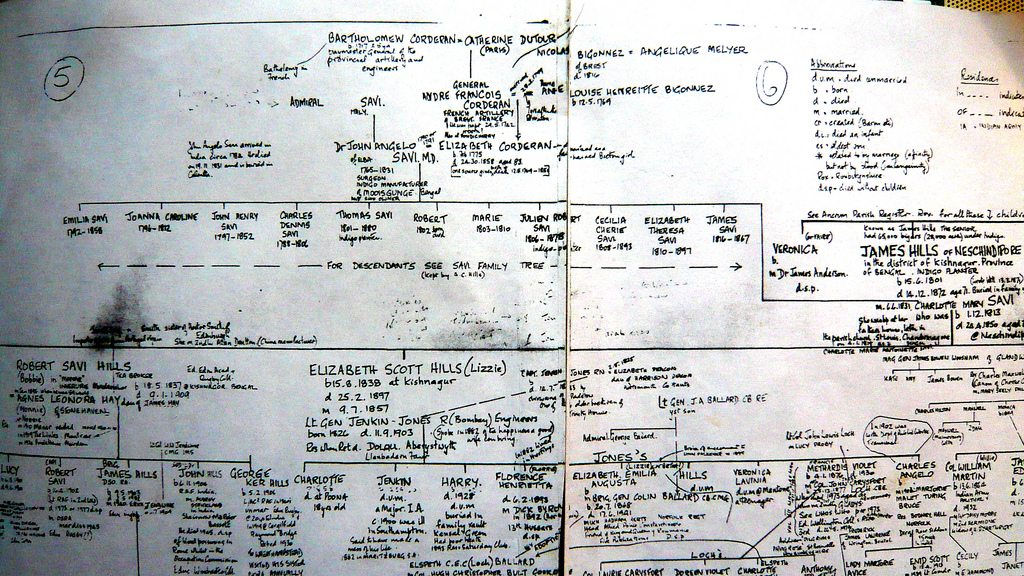
\includegraphics[width=0.8 \linewidth]{Figures/FamilyTree.jpg} \\
					\tiny{\url{https://www.flickr.com/photos/herry/3228640890}}
		\end{column}
		\begin{column}{0.4 \linewidth}
			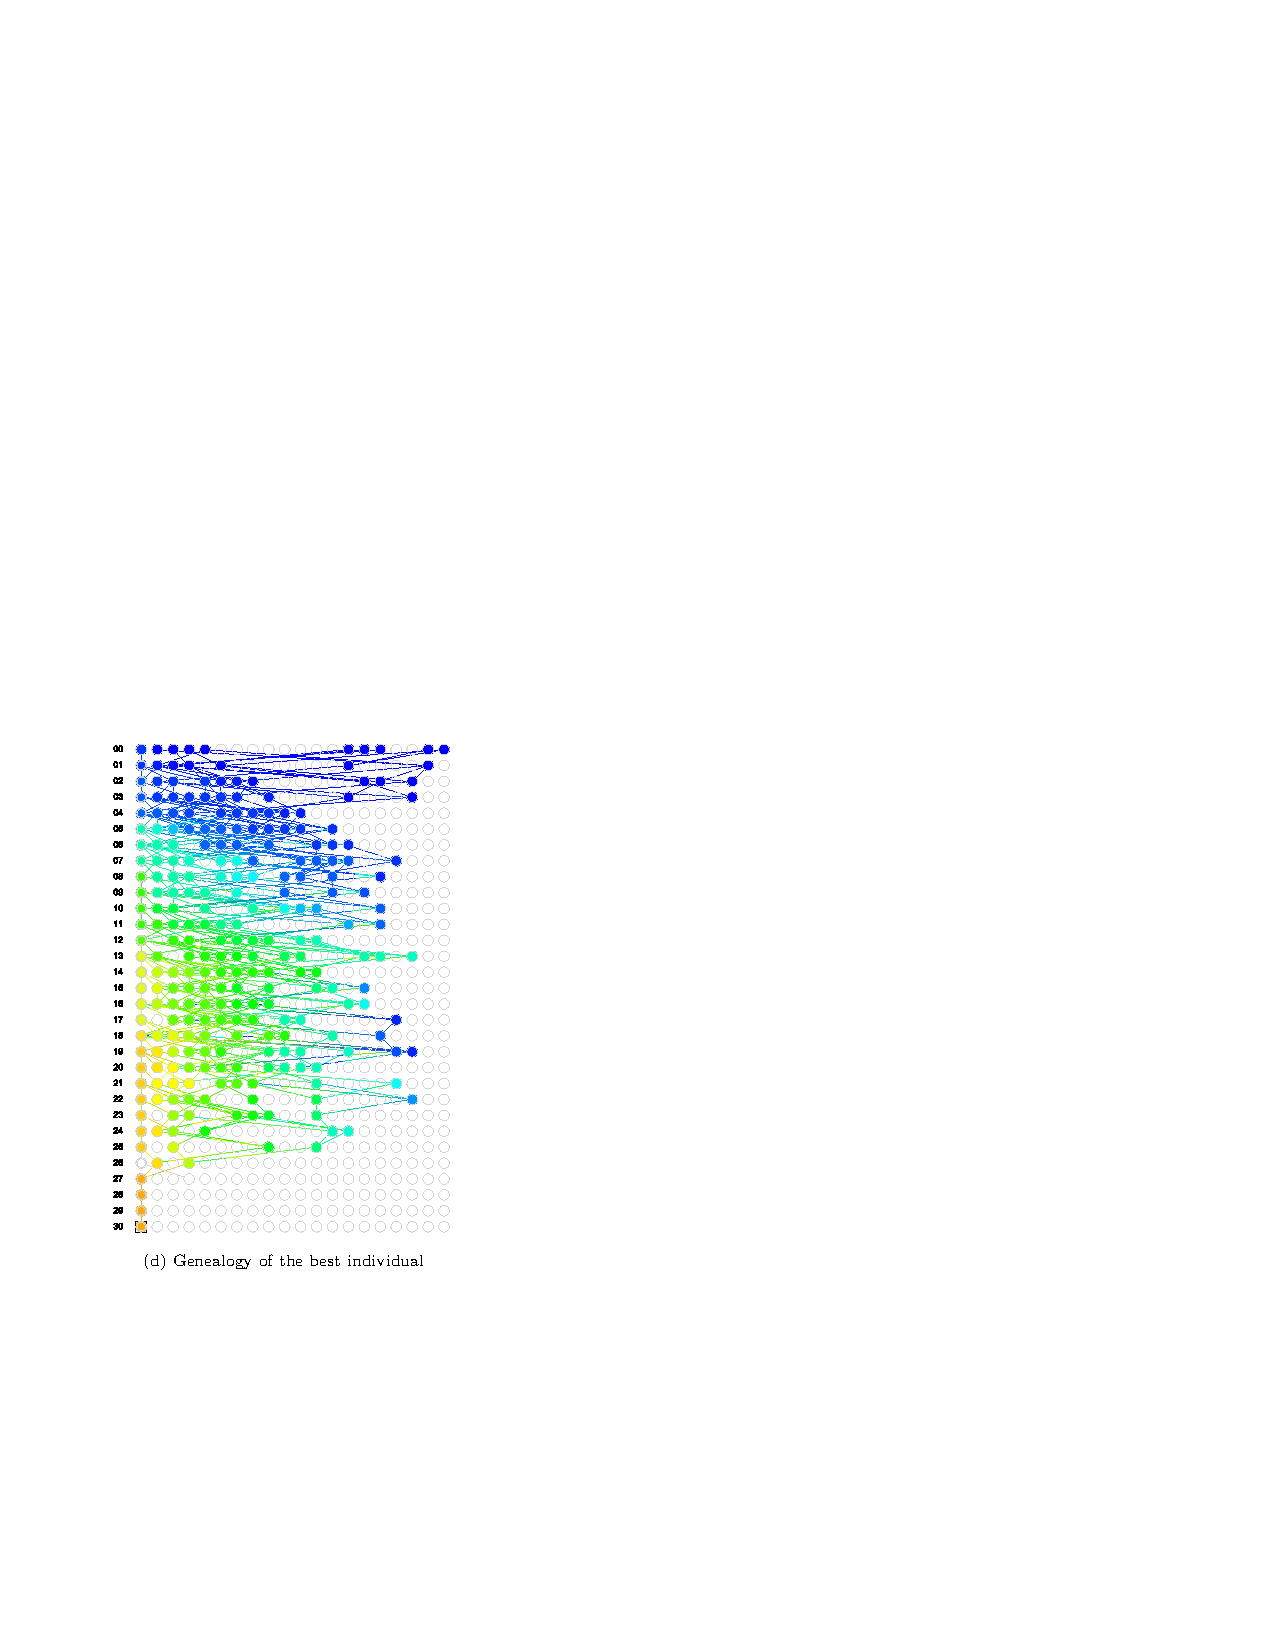
\includegraphics[height= 0.75 \textheight]{Figures/HeuristicLabGraph.pdf} \\
			\tiny{\cite{Burlacu:2013:VGL:2464576.2482714}}
		\end{column}		
	\end{columns}
\end{frame}

\subsection{Neo4j}

\begin{frame}{Neo4j graph database}
	
\begin{columns} 
\begin{column}{0.65 \textwidth}
		\begin{itemize}
			\item Part of the new-ish NoSQL movement
			\begin{itemize}
				\item Neo4j's initial release was 2007
				\item Started to take off in 2010
			\end{itemize}
			\item Easy to represent complex relationships
			\item Easy to \emph{search} for relationships
			\item Efficient recursive queries, esp. compared to traditional databases
		\end{itemize}
		\end{column}
		\begin{column}{0.35\textwidth}
			\centering
	   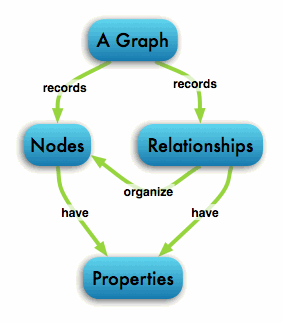
\includegraphics[width=0.95\textwidth]{Figures/graphdb-neo4j.png}
       \\
    \tiny{\url{http://neo4j.com}}
  \end{column}
  \end{columns}

\end{frame}

\subsection{Cypher}

\begin{frame}{Cypher query language}
	\begin{columns}
		\begin{column}{0.4\textwidth}
			Neo4j uses the \emph{Cypher} query language.

			\linespace
			
			Fundamental elements of Cypher queries:
		\begin{itemize}
			\item START
			\item MATCH
			\item WHERE
			\item RETURN
		\end{itemize}
		
		\linespace
		
		Uses "ASCII art" to describe relationships.
	\end{column}
	\begin{column}{0.60\textwidth}

	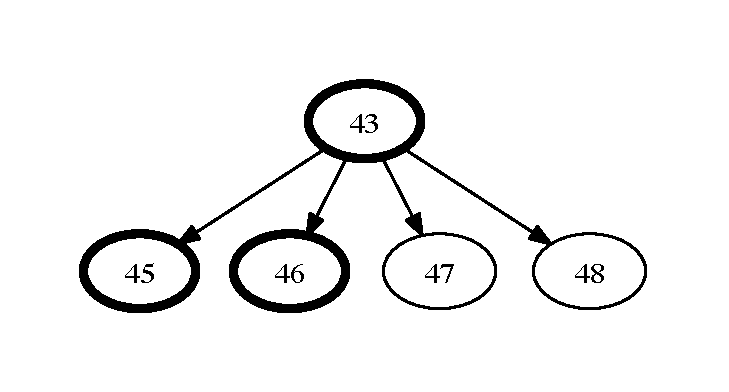
\includegraphics[width=.95\textwidth]{Figures/parents.pdf}
	\linebreak
	{
START parent=node(43)
\linebreak
MATCH (parent)-[:PARENTOF]->(child)
\linebreak
\textbf{WHERE id(child) < 47}
\linebreak
RETURN parent, child;
}

	\end{column}	
	\end{columns}
\end{frame}

\begin{frame}{Can model (more) arbitrary paths}
	Find all Nic's friends:
	
	\begin{center}
		\texttt{(Nic)-[:FRIEND\_OF]->(p)}
	\end{center}
	
	Find all the friends of Nic's friends:
	
	\begin{center}
		\texttt{(Nic)-[:FRIEND\_OF*2]->(p)}
	\end{center}
	
	Find everyone at most 5 steps from Nic:
	
	\begin{center}
		\texttt{(Nic)-[:FRIEND\_OF*1..5]->(p)}
	\end{center}
	
\end{frame}

\begin{frame}{Can model (more) arbitrary paths}
	Find all Nic's grandparents:
	
	\begin{center}
		\texttt{(Nic)<-[:PARENT\_OF*2]-(gp)}
	\end{center}
	
	Find all Nic's siblings:
	
	\begin{center}
		\texttt{(Nic)<-[:PARENT\_OF]-()-[:PARENT\_OF]->(s)}
	\end{center}
	
	Find all Nic's cousins (and siblings):
	
	\begin{center}
		\texttt{(Nic)<-[:PARENT\_OF*2]-()-[:PARENT\_OF*2]->(c)}
	\end{center}
	
\end{frame}

\section{Let's go exploring!}

\subsection{Setup}

\begin{frame}{What are we exploring?}
Tom Helmuth provided a \emph{lot} of data:
\begin{itemize}
	\item A number of program synthesis problems taken from intro computing texts
	\item Three different selection mechanisms: Lexicase, tournament, and implicit fitness sharing (IFS)
	\item All using Clojush implementation of Lee Spector's PushGP system \url{https://github.com/lspector/Clojush}
	\item Population size 1,000; $\leq 300$ generations
\end{itemize}
See \cite{Helmuth:GECCO15} for more.

\linespace

We used \texttt{batch-import} tool and custom scripts to import into Neo4j. 
{\tiny \url{https://github.com/jexp/batch-import}} 
\end{frame}

\begin{frame}{Only just the beginning}
	\begin{itemize}
		\item We have data from hundreds of runs
		\item Currently a very ``by hand'' process
		\item Definitely learned valuable things about:
		\begin{itemize}
			\item The behavior of lexicase
			\item Role of alternation (a type of crossover) in PushGP
			\item Impact of test cases on evolutionary dynamics
		\end{itemize}
	\end{itemize}
	
	\linespace
	
	We'll look at results from two runs:
	\begin{itemize}
		\item Both successful on replace-space-with-newline problem
		\item One using lexicase (sol'n found in 88 gens)
		\item One using tournament selection (sol'n found in 151 gens)
	\end{itemize}
\end{frame}

\subsection{Comparing the end-games}

\begin{frame}{How did we construct a winner?}
	How is a winner constructed at the end of a run?
	
	\linespace
	
	This query finds all ancestors of a winner (zero \texttt{total\_error}) going back at most 8 steps:
	
	\linespace
	
	\texttt{$\quad$ MATCH (w \{total\_error: 0\}) \\
		$\quad$ MATCH (p)-$\,$->(c)-[*0..7]->(w) \\
$\quad$ RETURN DISTINCT id(p), id(c);}

	\linespace
	
	8 steps is fairly arbitrary; returns a small enough set to visualize.
\end{frame}

\begin{frame}{Comparing the end-games}
	\begin{columns}
		\begin{column}{0.5 \linewidth}
			Ancestry of winner(s) look very different
			\begin{itemize}
				\item Tournament selection (below): Single winner w/ high branching factor
				\item Lexicase (right): 45 winners w/ much lower branching factor
			\end{itemize}
			\begin{center}
				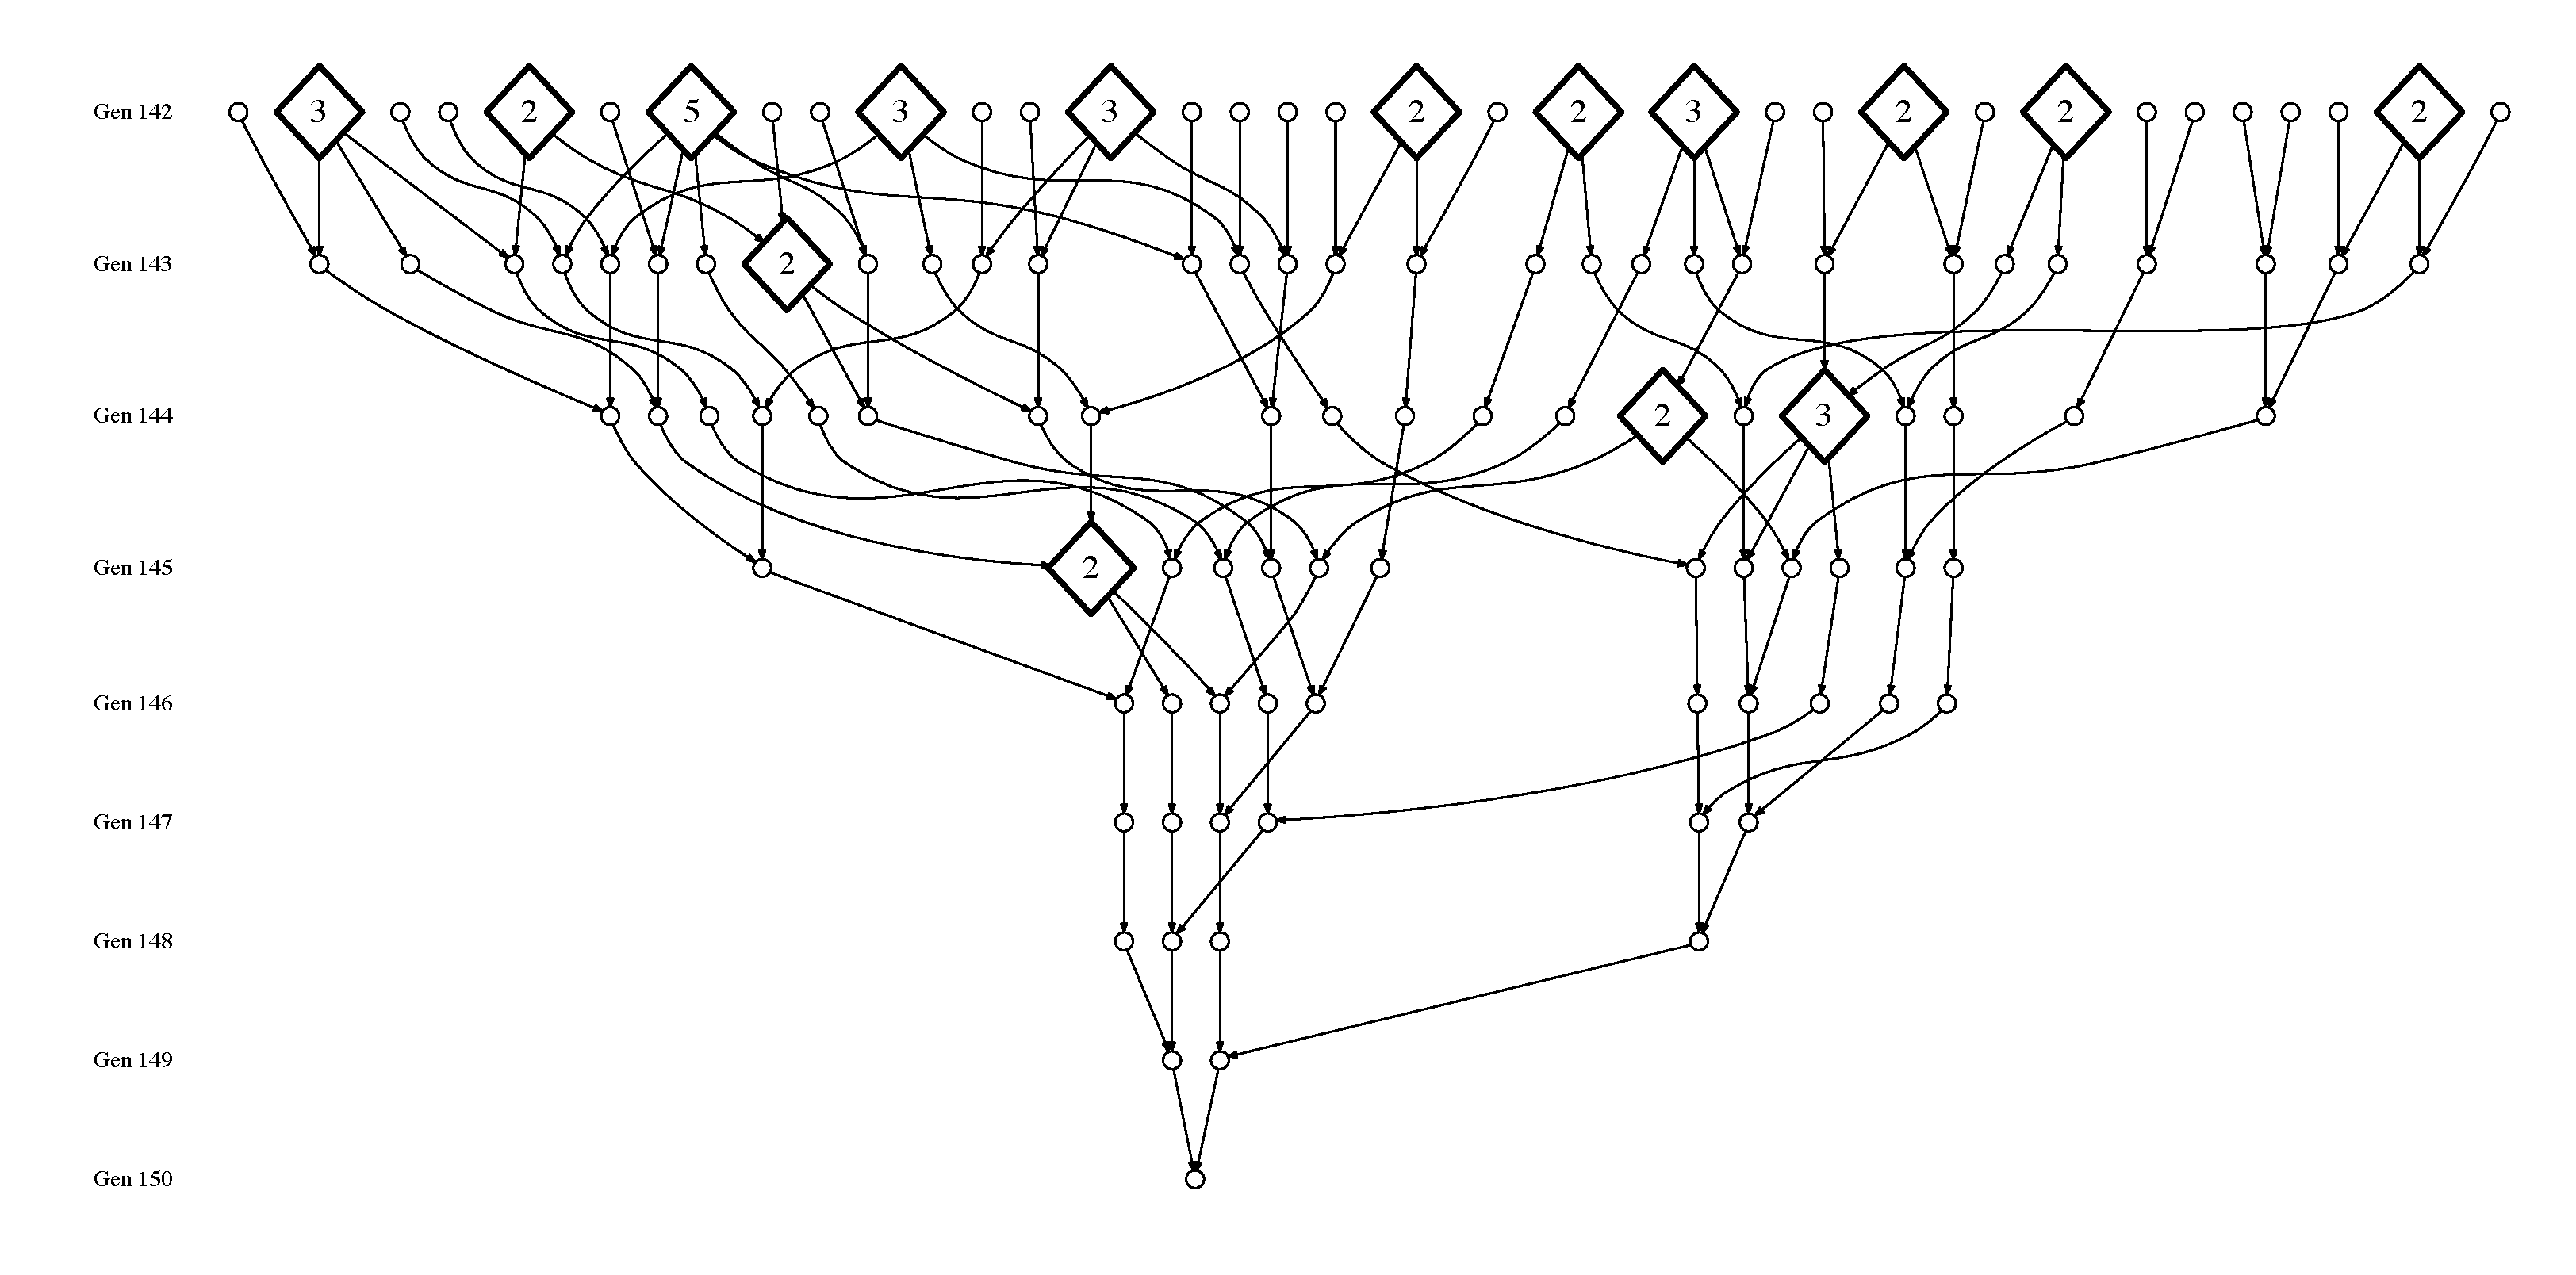
\includegraphics[width=\linewidth]{Figures/ancestors_of_winner_rswn_tourney_run74_9gens}
			\end{center}
		\end{column}
		\begin{column}{0.5 \linewidth}
			\begin{center}
				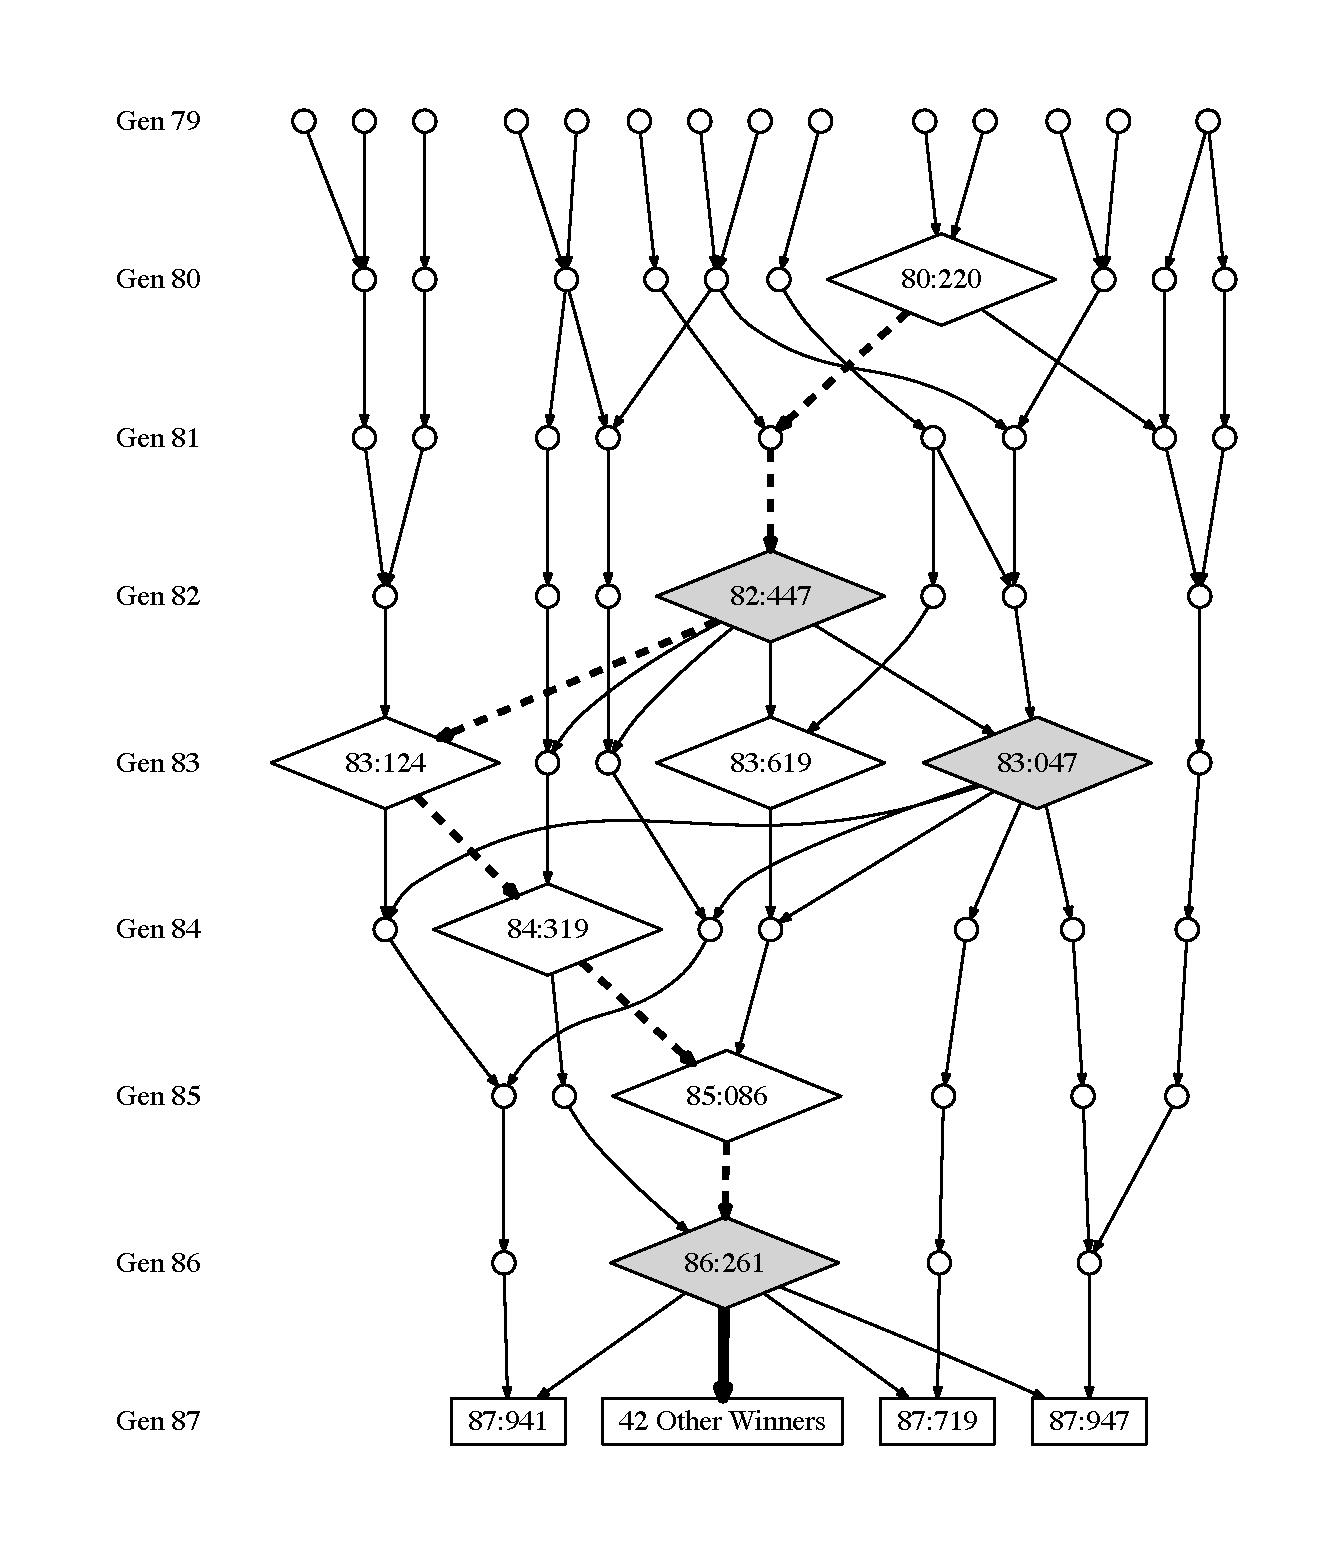
\includegraphics[width=\linewidth]{Figures/ancestors_of_winners_colons}
			\end{center}
		\end{column}
	\end{columns}
\end{frame}

\begin{frame}{Lexicase selection}
	\begin{columns}
		\begin{column}{0.5 \linewidth}
			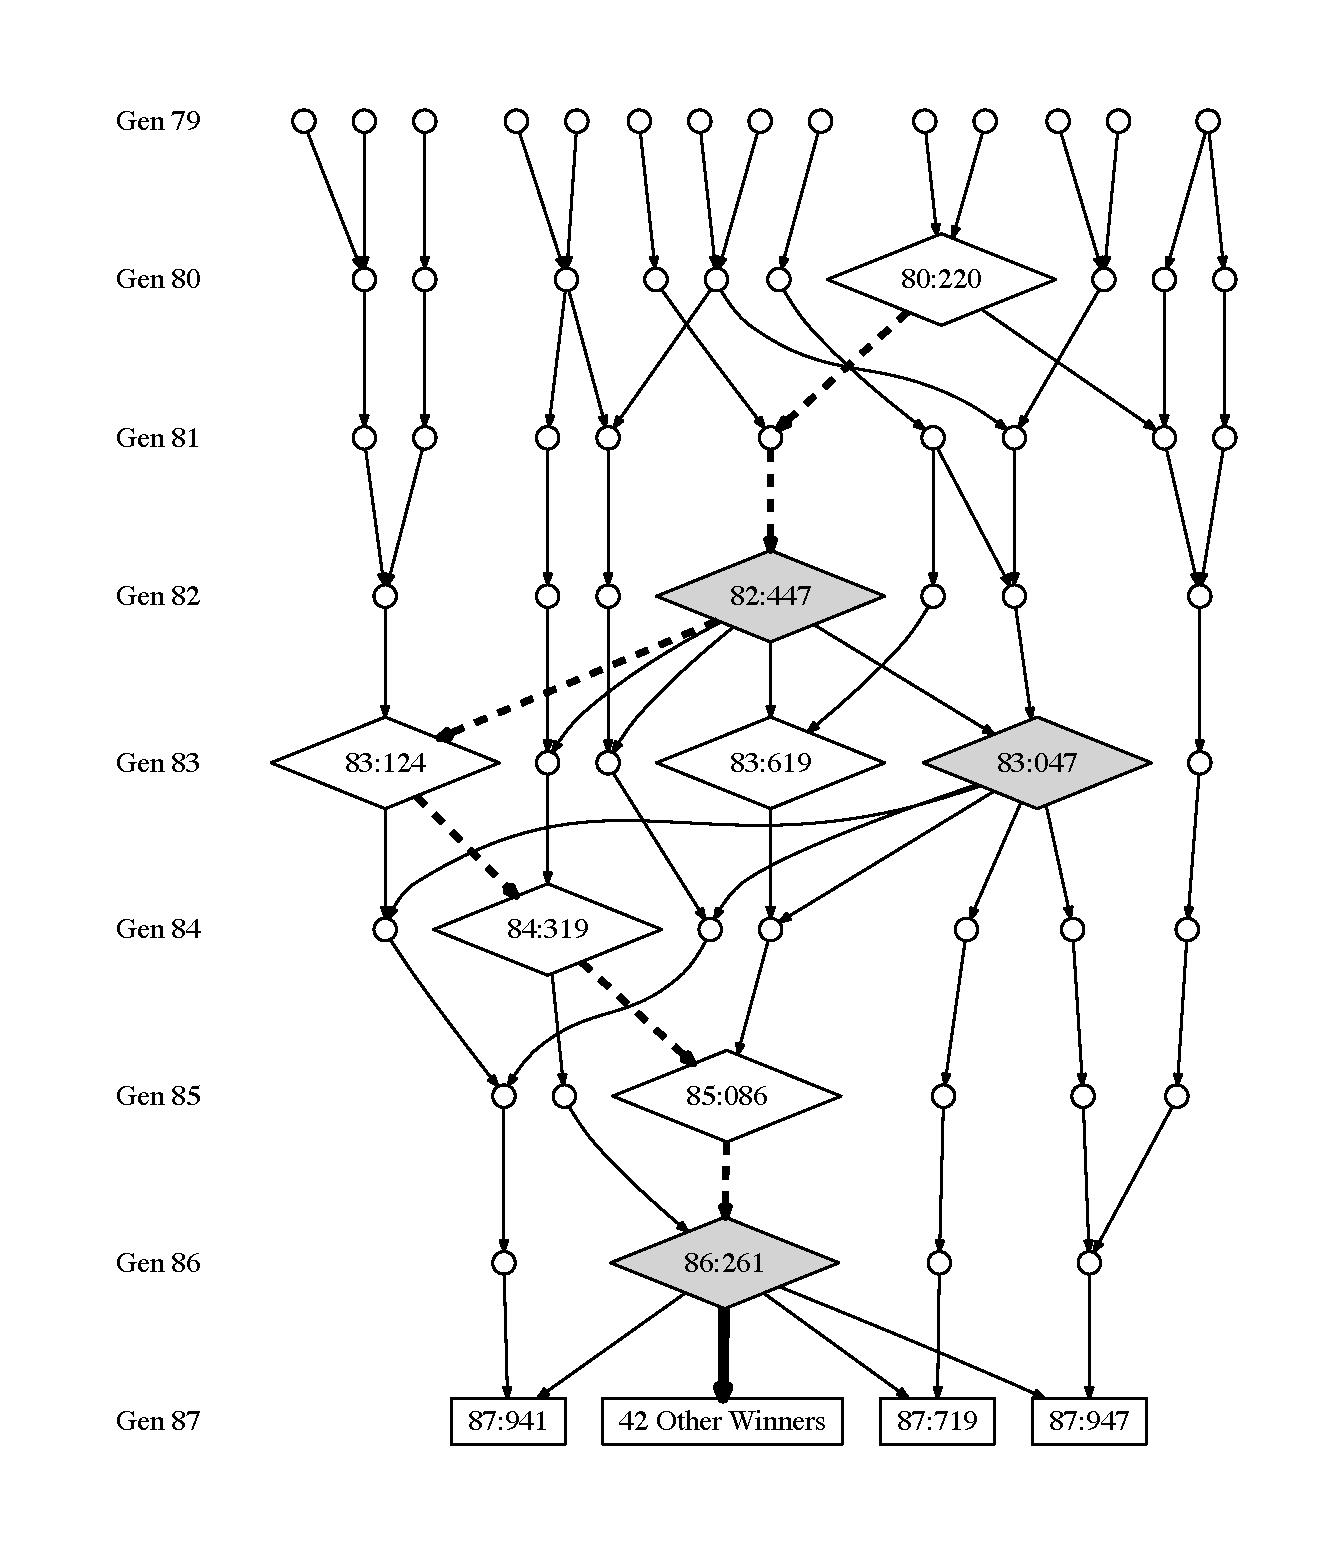
\includegraphics[height=0.9\textheight]{Figures/ancestors_of_winners_colons}
		\end{column}
		\begin{column}{0.45 \linewidth}
			\begin{overprint}
				\onslide<1>
			A number of observations:
			\begin{itemize}
				\item 45(!) ``winning'' individuals
				\item Individual ``86:261'' is (a) parent of all 45
				\item Individual ``86:261'' is a parent of 934 (of 1,000) individuals in next generation
			\end{itemize}
			
			\onslide<2>
			Seriously?!? 934 offspring?!?
			
			\linespace
			
			Turns out to an be extreme case of a common phenomena with lexicase
			
			\linespace
			
			Nodes marked with diamonds all had at least 100 offspring
			
			\linespace
			
			Shaded diamonds also have at least 5 offspring that are ancestors of or are winners
			
			\onslide<3-4>
			What's the total error (fitness) of ``86:261''?
			\begin{itemize}
				\item<4> 4,034(!)
				\item<4> Bottom quartile!
				\item<4> But had 934 offspring! \linespace
				\item<4> Failed to return on 4 cases (error 1,000 each)
				\item<4> Got 2 other answers wrong (error 17 each)
				\item<4> Terrible total error, but perfect on 194 of 200 tests
				\item<4> Great for lexicase!
			\end{itemize}
						
			\onslide<5-6>
			What's the total error (fitness) of ``85:086''?
			\begin{itemize}
				\item<6> \emph{100,000!}
				\item<6> Rank 971 out of 1,000
				\item<6> But had 180 offspring \linespace
				\item<6> Got all the ``print'' cases
				\item<6> Failed to return value for all 100 ``return'' cases (error 1,000 each)
				\item<6> \emph{Terrible} total error, but perfect on 100 of 200 tests
				\item<6> Fine for lexicase
			\end{itemize}
			
			\end{overprint}
		\end{column}
	\end{columns}
\end{frame}

\begin{frame}{Tournament selection}
	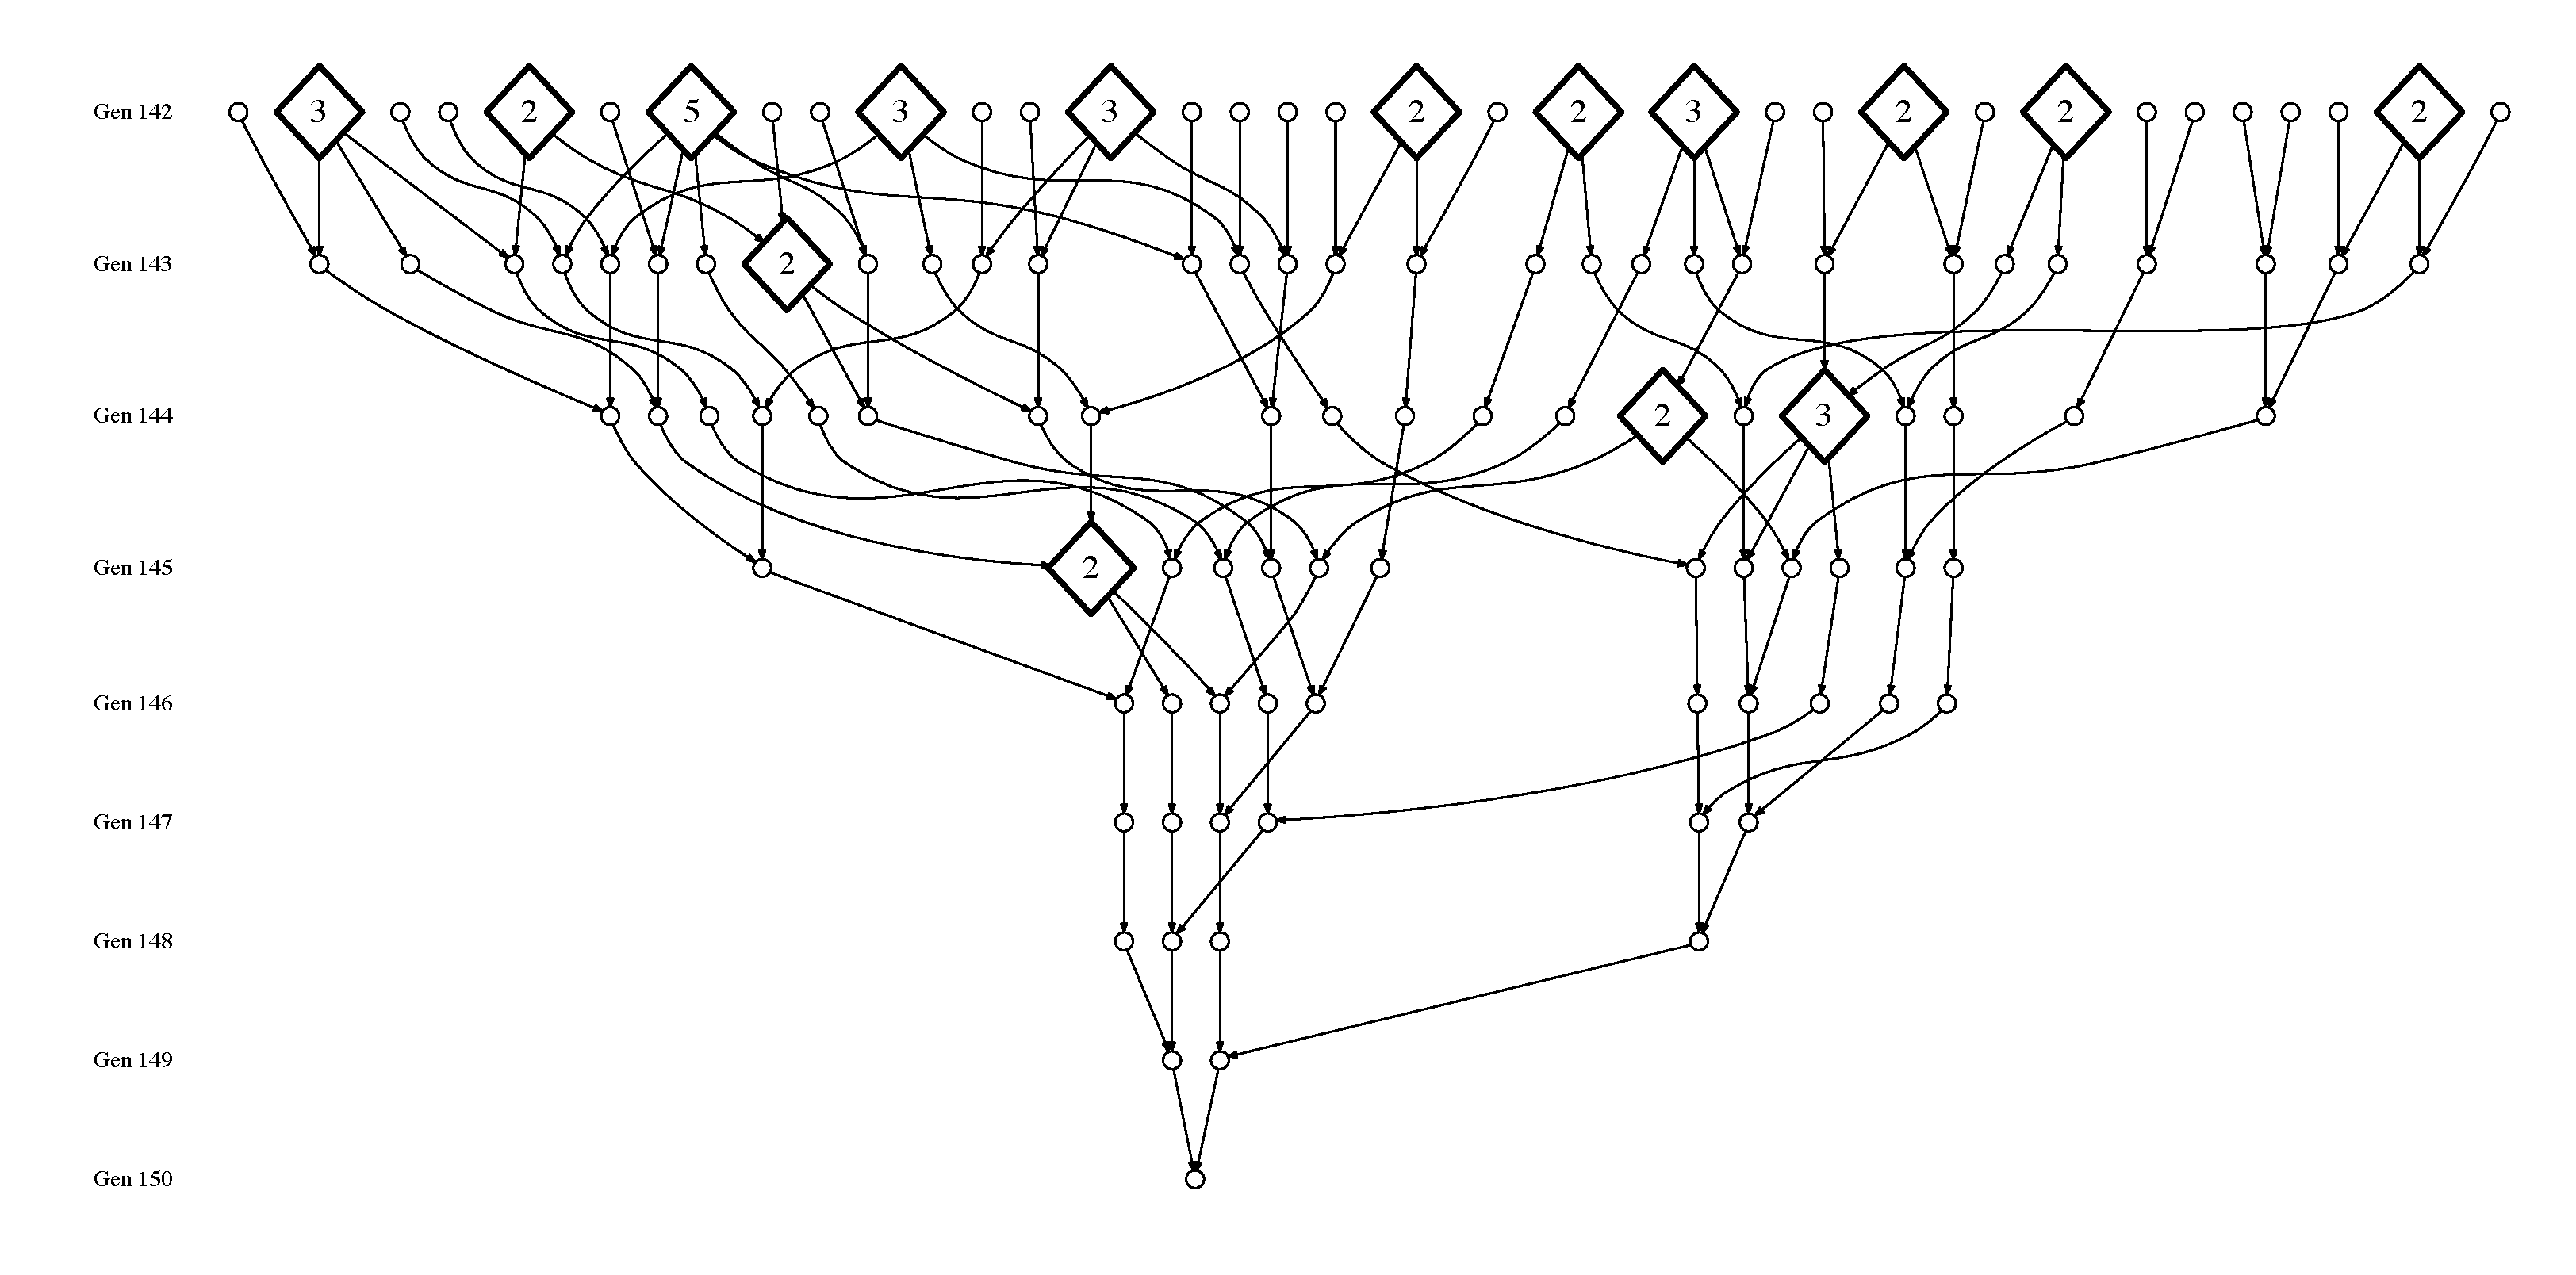
\includegraphics[width=\linewidth]{Figures/ancestors_of_winner_rswn_tourney_run74_9gens}
	
	Much broader: 42 ancestors of a winner for tournament 9 gens back; 14 for lexicase
\end{frame}

\begin{frame}{Number ancestors of ``winners'' over time}
		\begin{center}
			\begin{tabular}{rrr}
				Gens from winner & Lexicase & Tournament \\
				\hline\noalign{\smallskip}                
                1 & 4 & 2 \\
                2 & 6 & 4 \\
                3 & 7 & 6 \\
                4 & 6 & 10 \\
                5 & 7 & 13 \\
                6 & 9 & 20 \\
                7 & 10 & 30 \\
                8 & 14 & 33 \\
                9 & 14 & 42 \\
                10 & 22 & 63 \\ 
%                \ldots \\
%                15 & 49 & 152 \\
                \ldots \\ 
                18 & 58 & 297 \\
			\end{tabular}
		\end{center}
\end{frame}

\begin{frame}{Most fecund individuals}
		\begin{center}
			\begin{tabular}{rrr}
				Fecundity rank & Lexicase & Tournament \\
				\hline\noalign{\smallskip}
				1 & 934 & 24 \\
				2 & 657 & 23 \\
				3 & 594 & 23 \\
				4 & 590 & 21 \\
				5 & 433 & 20 \\
				6 & 326 & 20 \\
				7 & 297 & 19 \\
				8 & 294 & 19 \\
				9 & 285 & 19 \\
				10 & 283 & 18 \\
				11 & 279 & 18 \\
				12 & 271 & 18 \\
			\end{tabular}
		\end{center}
\end{frame}

\section[Results]{Results}

\subsection[Questions Asked]{Questions Asked}

\begin{frame}
\frametitle{Questions Asked}
\begin{enumerate}
\item \emph{What does the fitness of the ``winning'' individual's ancestry line look like over time?}
\item \emph{How often does mutation improve fitness? Also, how often does crossover improve fitness, where the root parent is more fit than the non-root parent, and vice versa?}
\item \emph{Does a group of individuals have a common root parent ancestor and what is the latest generation where such an ancestor occurs?}
\item \emph{How many individuals in the initial generation have any root parent descendants in the final generation?}
\end{enumerate}
\end{frame}

\subsection[Fitness Graph]{Fitness Over Time}

\begin{frame}
\frametitle{Fitness Over Time}
\emph{What does the fitness of the ``winning'' individual's ancestry line look like over time?}
\begin{center}
% \includegraphics[width=0.85\textwidth]{Combined_fitness_over_time_no_dashed}
\end{center}
\end{frame}

\subsection[Improved Transformations]{Improved Transformations}

\begin{frame}
\frametitle{Percentage of Improved Transformations}
\emph{How often does mutation and crossover improve fitness?}
\begin{center}
{\tiny Results for Three 1,000 Individual Runs and One 10,000 Individual Run}
% \includegraphics[width=0.95\textwidth]{All_percentages_over_time}
\end{center}
\end{frame}

\subsection[Common Ancestor]{Common Ancestor}

\begin{frame}
\frametitle{Common Ancestor}
\emph{Does a group of individuals have a common root parent ancestor and how many initial generation individuals have descendants in the final generation?}
\begin{center}
% \includegraphics[height=0.70\textheight]{subset_confluence_trimmed}
\end{center}

\end{frame}

\section[Conclusions]{Conclusions}

\begin{frame}
\frametitle{Conclusions}

\begin{itemize}
\item We can gather internal data efficiently.
\item Provides more in depth information than statistical summaries. 
\item Support for hypotheses.
\end{itemize}
\linespace
\linespace
\linespace
\linespace

Future Work
\begin{itemize}
\item Trying different setup configurations.
\item Enforcing the root parent to have better fitness in XO.
\item Dynamically change parameters.
\end{itemize}
\end{frame}

\begin{frame}{Thanks!}
	
	Thank you for your time and attention!

	\linespace
	
	Thanks to M. Kirbie Dramdahl (University of Minnesota, Morris), and to Lee Spector's Computational Intelligence group (Hampshire College) for ideas and feedback.
	
	\linespace
	
	Contacts:  
	\begin{itemize}
		\item \texttt{mcphee@morris.umn.edu}
		\item \texttt{donat056@morris.umn.edu}
		\item \texttt{thelmuth@cs.umass.edu}
	\end{itemize}
	
	\linespace
	\linespace
	
	\begin{center}
	{\huge Questions?}
	\end{center}
\end{frame}

\section*{References}

\begin{frame} 
\frametitle{References}
\bibliographystyle{apalike}
{\tiny \bibliography{GraphDBandGP}}
\end{frame} 

\end{document}


